\documentclass[12pt,a4paper]{report}%
\usepackage[T1]{fontenc}%
\usepackage[utf8]{inputenc}%
\usepackage{lmodern}%
\usepackage{textcomp}%
\usepackage{lastpage}%
\usepackage[margin=1in]{geometry}%
\usepackage{graphicx}%
\usepackage{float}%
\usepackage{booktabs}%
\usepackage{array}%
\usepackage{setspace}%
\usepackage{parskip}%
\usepackage{titlesec}%
\usepackage{fancyhdr}%
\usepackage{needspace}%
\usepackage[table]{xcolor}%
\usepackage{tikz}%
\usepackage{pgfplots}%
\usepackage{hyperref}%
\usepackage{microtype}%
%
\pgfplotsset{compat=1.18}%

\hypersetup{
  colorlinks=true,
  linkcolor=black,
  urlcolor=black,
  citecolor=black
}
%
\onehalfspacing%
\setlength{\parindent}{0pt}%
\setlength{\parskip}{9pt}%
\setlength{\textfloatsep}{16pt}%
\setlength{\intextsep}{16pt}%
\setlength{\abovecaptionskip}{6pt}%
\setlength{\belowcaptionskip}{6pt}%
\renewcommand{\contentsname}{Table of Contents}%

\titleformat{\section}{\Large\bfseries}{\thesection.}{0.9em}{}
\titleformat{\subsection}{\large\bfseries}{\thesubsection}{0.9em}{}
\titlespacing*{\section}{0pt}{22pt}{10pt}
\titlespacing*{\subsection}{0pt}{14pt}{8pt}
%
\setlength{\headheight}{15pt}%

\pagestyle{fancy}
\fancyhf{}
\lhead{\textbf{Simply Supported Beam Analysis Report}}
\rhead{\textbf{Soniya Kuchekar}}
\cfoot{Page \thepage\ of \pageref{LastPage}}
\renewcommand{\headrulewidth}{0.4pt}
\renewcommand{\footrulewidth}{0.4pt}
%
%
\begin{document}%
\normalsize%
\thispagestyle{empty}%
\begin{tikzpicture}[remember picture,overlay]%
\fill[black!6] (current page.north west) rectangle ([yshift=-3.8cm]current page.north east);%
\fill[black!22] (current page.north west) rectangle ([xshift=0.35cm,yshift=-3.8cm]current page.north west);%
\end{tikzpicture}%
\vspace*{2.2cm}%
\begin{center}%
{\Huge\bfseries Simply Supported Beam Analysis Report}\\[0.35cm]%
{\Large Structural Beam Analysis using TikZ/pgfplots}\\[0.35cm]%
{\large VIT Bhopal University}\\[0.9cm]%
\rule{0.74\textwidth}{0.7pt}\\[0.7cm]%
{\Large \textbf{Author:} Soniya Kuchekar}\\[0.25cm]%
{\large \textbf{Report ID:} BA-2026-SONIYA-KUCHEKAR-SSB}\\[0.25cm]%
{\large \textbf{Date:} \today}%
\end{center}%
\vfill%
\newpage%
\tableofcontents%
\newpage%
\section{Introduction}%
\label{sec:Introduction}%
\vspace{-2pt}%
\textit{This section describes the beam system and the origin of the input dataset used for analysis.}%
\vspace{6pt}%
\subsection{Beam Description}%
\label{subsec:BeamDescription}%
The structure considered is a simply supported beam with a pinned support at the left end and a roller support at the right end. This arrangement allows rotation at both supports while preventing vertical displacement.%


\begin{figure}[H]%
\centering%
\includegraphics[width=0.82\textwidth]{beam.png}%
\caption{Simply Supported Beam Configuration}%
\end{figure}

%
\subsection{Data Source}%
\label{subsec:DataSource}%
The force and moment values used in this report are read directly from the provided Excel file (beam\_data.xlsx). The next section recreates the Excel table using LaTeX Tabular.

%
\section{Input Data}%
\label{sec:InputData}%
\vspace{-2pt}%
\textit{This section recreates the Excel dataset using a LaTeX table (not inserted as an image).}%
\vspace{6pt}%
\renewcommand{\arraystretch}{1.25}%
\rowcolors{2}{black!4}{white}%
\begin{center}%
\begin{tabular}{@{}>{\centering\arraybackslash}p{3.7cm}>{\centering\arraybackslash}p{5.3cm}>{\centering\arraybackslash}p{5.3cm}@{}}%
\toprule%
\textbf{Position (m)}&\textbf{Shear Force (kN)}&\textbf{Bending Moment (kNm)}\\%
\midrule%
0.00&45.00&0.00\\%
1.50&36.00&60.75\\%
3.00&27.00&108.00\\%
4.50&18.00&141.75\\%
6.00&9.00&162.00\\%
7.50&0.00&168.75\\%
9.00&{-}9.00&162.00\\%
10.50&{-}18.00&141.75\\%
12.00&27.00&108.00\\%
13.50&{-}36.00&60.75\\%
15.00&{-}45.00&0.00\\%
\bottomrule%
\end{tabular}%
\end{center}%
\rowcolors{2}{}{}

%
\section{Analysis}%
\label{sec:Analysis}%
\vspace{-2pt}%
\textit{This section presents engineering diagrams generated as TikZ/pgfplots vector plots for high-quality output.}%
\vspace{6pt}%
\Needspace{16\baselineskip}%
\subsection{Shear Force Diagram}%
\label{subsec:ShearForceDiagram}%
\begin{samepage}%
The Shear Force Diagram (SFD) illustrates the variation of shear force along the beam span.%

\begin{figure}[H]
\centering
\vspace{2mm}
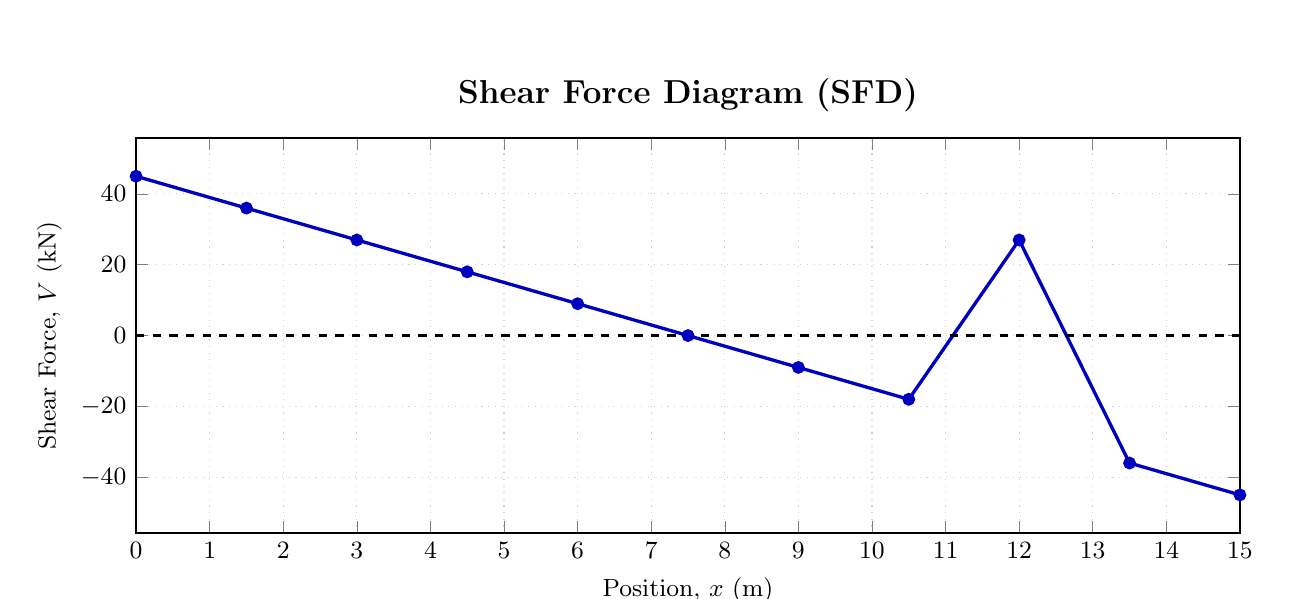
\begin{tikzpicture}
\begin{axis}[
    width=15.6cm,
    height=6.6cm,
    title={\textbf{Shear Force Diagram (SFD)}},
    title style={font=\large},
    xlabel={Position, $x$ (m)},
    ylabel={Shear Force, $V$ (kN)},
    xmin=0, xmax=15.00,
    ymin=-55.80, ymax=55.80,
    grid=major,
    grid style={dotted, gray!35},
    axis line style={black, thick},
    tick label style={font=\small},
    label style={font=\small},
]
\addplot[blue!75!black, very thick, mark=*, mark size=1.7pt]
coordinates {
(0.0, 45.0)
(1.5, 36.0)
(3.0, 27.0)
(4.5, 18.0)
(6.0, 9.0)
(7.5, 0.0)
(9.0, -9.0)
(10.5, -18.0)
(12.0, 27.0)
(13.5, -36.0)
(15.0, -45.0)
};
\addplot[black, dashed, thick] coordinates {(0,0) (15.00,0)};
\end{axis}
\end{tikzpicture}
\vspace{-2mm}
\end{figure}
%
\end{samepage}

%
\Needspace{16\baselineskip}%
\subsection{Bending Moment Diagram}%
\label{subsec:BendingMomentDiagram}%
\begin{samepage}%
The Bending Moment Diagram (BMD) represents the bending moment distribution along the span.%

\begin{figure}[H]
\centering
\vspace{2mm}
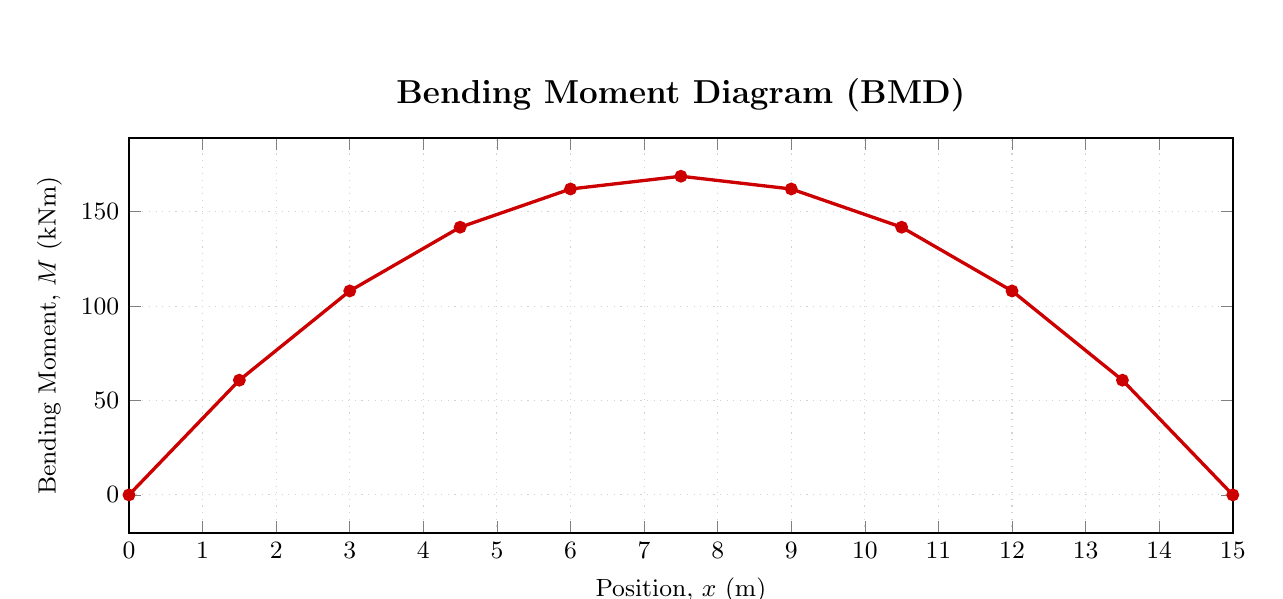
\begin{tikzpicture}
\begin{axis}[
    width=15.6cm,
    height=6.6cm,
    title={\textbf{Bending Moment Diagram (BMD)}},
    title style={font=\large},
    xlabel={Position, $x$ (m)},
    ylabel={Bending Moment, $M$ (kNm)},
    xmin=0, xmax=15.00,
    ymin=-20.25, ymax=189.00,
    grid=major,
    grid style={dotted, gray!35},
    axis line style={black, thick},
    tick label style={font=\small},
    label style={font=\small},
]
\addplot[red!80!black, very thick, mark=*, mark size=1.7pt]
coordinates {
(0.0, 0.0)
(1.5, 60.75)
(3.0, 108.0)
(4.5, 141.75)
(6.0, 162.0)
(7.5, 168.75)
(9.0, 162.0)
(10.5, 141.75)
(12.0, 108.0)
(13.5, 60.75)
(15.0, 0.0)
};
\end{axis}
\end{tikzpicture}
\vspace{-2mm}
\end{figure}
%
\end{samepage}

%
\end{document}